\subsection{Интернет вещей и мобильные приложения: влияние и взаимодействие}
\label{sec:subject:mobile}

Мобильное приложение~--- программное обеспечение, предназначенное для работы на смартфонах, планшетах и других мобильных устройствах. Многие мобильные приложения предустановлены на самом устройстве или могут быть загружены на него из онлайновых магазинов приложений, таких как App Store, BlackBerry App World, Google Play, 1mobile market, Windows Phone Store, Яндекс.store и других, бесплатно или за плату \cite{wiki_mobile_def}.

На сегодняшний день существует огромное количество разнообразных приложений, загружаемых в мобильный телефон. Все приложения можно условно разделить на развлекательные (игры, плееры, «читалки»), коммуникационные (мессенджеры, навигационные (карты), справочные (словари, базы данных) и прикладные (все от калькулятора до графических программ) \cite{mobile_business}.

Мобильные технологии имеют ряд неоспоримых преимуществ перед любыми другими видами маркетинговых коммуникаций. Использование в своем приложении функций игрового характера позволяет привлечь большую аудиторию, заинтересовав ее. Вы можете получать отзывы напрямую от своих клиентов, без посредников (таких, как интернет-сайты или ваши сотрудники) и прямо в момент совершения покупки.

Возможности мобильных приложений практически безграничны, но немало программ удаляются пользователем уже через пару суток после установки. Так что к разработке мобильного приложения стоит относиться серьезно и ответственно, как и к любому другому инструменту маркетинга.

В 2012 году рынок мобильных приложений оценивался в 53 миллиарда долларов, а прогноз на 2016 год гласил, что предполагаемый рост составит около 100 миллиардов долларов. Эти цифры немного отличаются у разных исследователей, но очевидным остается то, что мобильный рынок действительно масштабен. Доход разработчики получают с помощью внутренних in-app покупок, рекламы внутри приложений, а также сбора больших данных (big data). Самые многообещающие категории – это социальные сети, производительность, рекламные сервисы, а также полезные приложения для различных целей. Самые быстрорастущие рынки – Юго-Восточная Азия и Латинская Америка \cite{mobile_market}.

В США, 67~\% пользователей используют смартфон, чтобы выходить в интернет каждый день, и большинство никогда не выйдут из дома без своего телефона. Аналогичный рост использования смартфонов наблюдается и в России – даже пользователи с доходами ниже среднего чаще выбирают смартфон вместо компьютера, чтобы всегда оставаться на связи с миром. Исследования рынка показывают, что около половины всех пользователей мобильных телефонов загрузили приложения, а две трети из них регулярно их используют. Большинство пользователей мобильных приложений находятся в возрастном промежутке от 25 до 30 лет, женаты или замужем, живут в пригородных районах, и имеют высшее образование. Таким образом, пользователи мобильных приложений в целом моложе, более образованы и имеют более высокий доход, нежели пользователи, не использующие мобильные приложения \cite{mobile_market}.

Две операционные системы Android и iOS доминируют на мобильном рынке. У Apple и Google два самых популярных магазина приложений, и сегодня кажется, что другим участникам рынка можно даже не мечтать, чтобы пробиться к лидерству.

Есть интересная статистика среднемесячного дохода, который приносили мобильные приложения. Статистику привел иностранный Forbes. Итак, в 2013-м году iOS приносила своим разработчикам в среднем \$4 000 в месяц, на втором месте был Android с его \$1 125, и аутсайдером был Windows Phone и всего \$625 \cite{mobile_tendency}.

В 2016-м году ситуация поменялась. Согласно данным Statista, приложение Windows Phone приносит, в среднем, \$11 400 в месяц, тогда как приложение iOS генерирует \$8 100, а Android — \$4 900. При этом 75~\% разработчиков являются приверженцами Android \cite{mobile_tendency}.

Пользовательские приложения для Интернета вещей можно разделить на две большие группы по их назначению:
\begin{itemize}
    \item Приложения для сбора и анализа данных – их главная задача заключается в снятии показаний с устройства и сохранении их в приложении (приложения для фитнес-трекеров, весов, измерителей влажности, камер, нитратомеров и т.д.);
    \item Приложения для управления – они способны не только проследить за устройством, но и изменить его состояние (приложения для кофеварок, чайников, умного дома и т.д.).
\end{itemize}

Приложения, как и сами IoT устройства, можно отнести к какой-либо категории – «фитнес и здоровье», «медицина», «бытовая техника», «мультимедиа», «умный дом». Все зависит от того, каким устройством оно управляет. В любом случае, если этот девайс есть в продаже, то приложение к нему можно скачать в PlayMarket и AppStore абсолютно бесплатно. Обычно такие приложения очень просты в использовании, причем, как правило, одно приложение создается на всю линейку техники одного производителя, а пользователь уже синхронизирует те устройства, которые имеются у него. Конечно, можно загрузить данное приложение и без устройства, но в таком случае оно будет бесполезно, так как сразу потребует подключить к нему гаджет \cite{mobile_apps_iot}.

Рассмотрим функциональные возможности некоторых пользовательских IoT приложений. Многие «умные» устройства категории «фитнес и здоровье» отслеживают различные физиологические показатели организма. К примеру, глюкометр iHealth Smart Glucometer, разработанный компанией iHealth Labs Inc., может контролировать уровень сахара в крови и пересылать результаты измерений на смартфон, в приложение iHealth Gluco-Smart (Рисунок~\ref{fig:subject:mobile:iHealth}). Данные измерений могут быть сохранены в само устройство (около 500 измерений) или, если смартфон под рукой, сразу в мобильное приложение. Кроме того собранную информацию можно загрузить в облачное хранилище, предоставляемое пользователям бесплатно.

В данном приложении можно следить за изменением уровня сахара в течение дня, недели, месяца и т.д., контролировать срок годности тестовых полосок, устанавливать напоминания о необходимости измерений уровня сахара или приеме лекарств, отправлять статистику измерений (в виде графика или таблицы) на электронную почту или делиться результатами в социальных сетях. Информация передается на мобильное устройство по Bluetooth. К результатам измерений можно добавлять голосовые и текстовые заметки о питании, занятиях спортом, количестве углеводов в пище и многое другое \cite{mobile_apps_iot}.

~
\begin{figure}[H]
\centering
	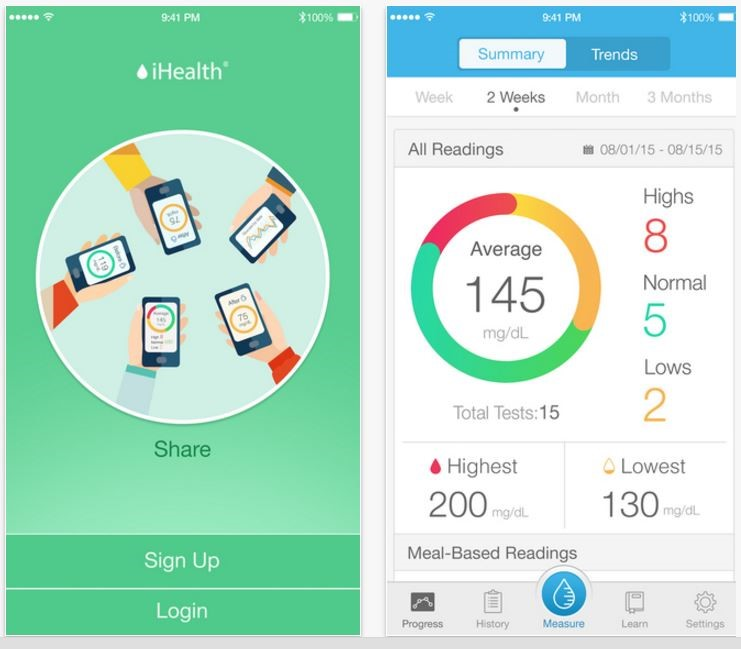
\includegraphics[scale=0.8]{figures/iHealth.jpg}
	\caption{Мобильное приложение для управления мультиварками Redmond}
	\label{fig:subject:mobile:iHealth}
\end{figure}

Все это говорит нам о том, что рынок мобильных приложений является очень перспективным и быстрорастущим. Мобильные приложения очень помогают в продвижении товара. Также они очень удобны как для пользователя, так и для разработчика, так как предоставляют большой спектр всевозможных датчиков и сетевых возможностей. Теперь понятно, что управление световым оборудованием с помощью именно мобильного приложения, это самый логичный и верный вариант для выбора вектора развития производства светового оборудования.